\subsection{Distributed approach}
\label{subsec:ex1distr}

\subsubsection{Model training}
\label{subsubsec:learneddist}

Once, enough data are collected through the simulator by using the optimal 
controller, it is possible to train a very simplified ``distributed network'' 
that takes as input an array containing the response values of the sensors – 
which can be either \texttt{prox\_values}, \texttt{prox\_comm} or 
\texttt{all\_sensors} – and produces as output an array containing one float 
that represents the speed of the wheels, which is assumed to be the same 
both right and left.

The dataset then contains a fixed number of simulation runs, each of these 
composed by a variable quantity of timesteps. It is important to notice that 
for this approach, unlike the one with communication, it is not necessary to 
keep the order of the sequence of timesteps, neither to know the exact 
number of agents in the simulation since the network input is the sensing 
associated to a single robot.

For this reason, the model is independent of the number of agents and 
consequently it is possible to prove its generalisation capacity, regardless 
the number of robots, by training the networks first on datasets each with a 
different but fixed value of $N$ and then on simulations composed by a 
variable $N$.
It is easy to show that although the value of $N$ changes the network 
structure does not, as it is sufficient during the input preprocessing to 
change the dimension of the input in such a way that all the tensors have 
the same length, fixed at the maximum possible value of $N$, padding 
those tensors with a lower number of agents.

Thanks to these two assumptions, it is possible to shuffle the original 
dataset, based on the single run, in order to improve the generalisation on 
the samples, and then split the resulting collection into the train, the 
validation and the test sets, containing respectively $60$-$20$-$20\%$ of 
the data. 

The architecture of the network, displayed in Figure 
\ref{fig:singlenetdistributed1}, is straightforward: there are three linear 
layers each of size $\langle\mathtt{input\_size}, 10\rangle$,  $\langle 10, 
10\rangle$ and $\langle 10, 1\rangle$, where \texttt{input\_size} is the 
shape of the sensing, that can be $7$ or $14$.
\begin{figure}[htb]
	\centering
	\begin{subfigure}[h]{0.495\textwidth}
		\centering
		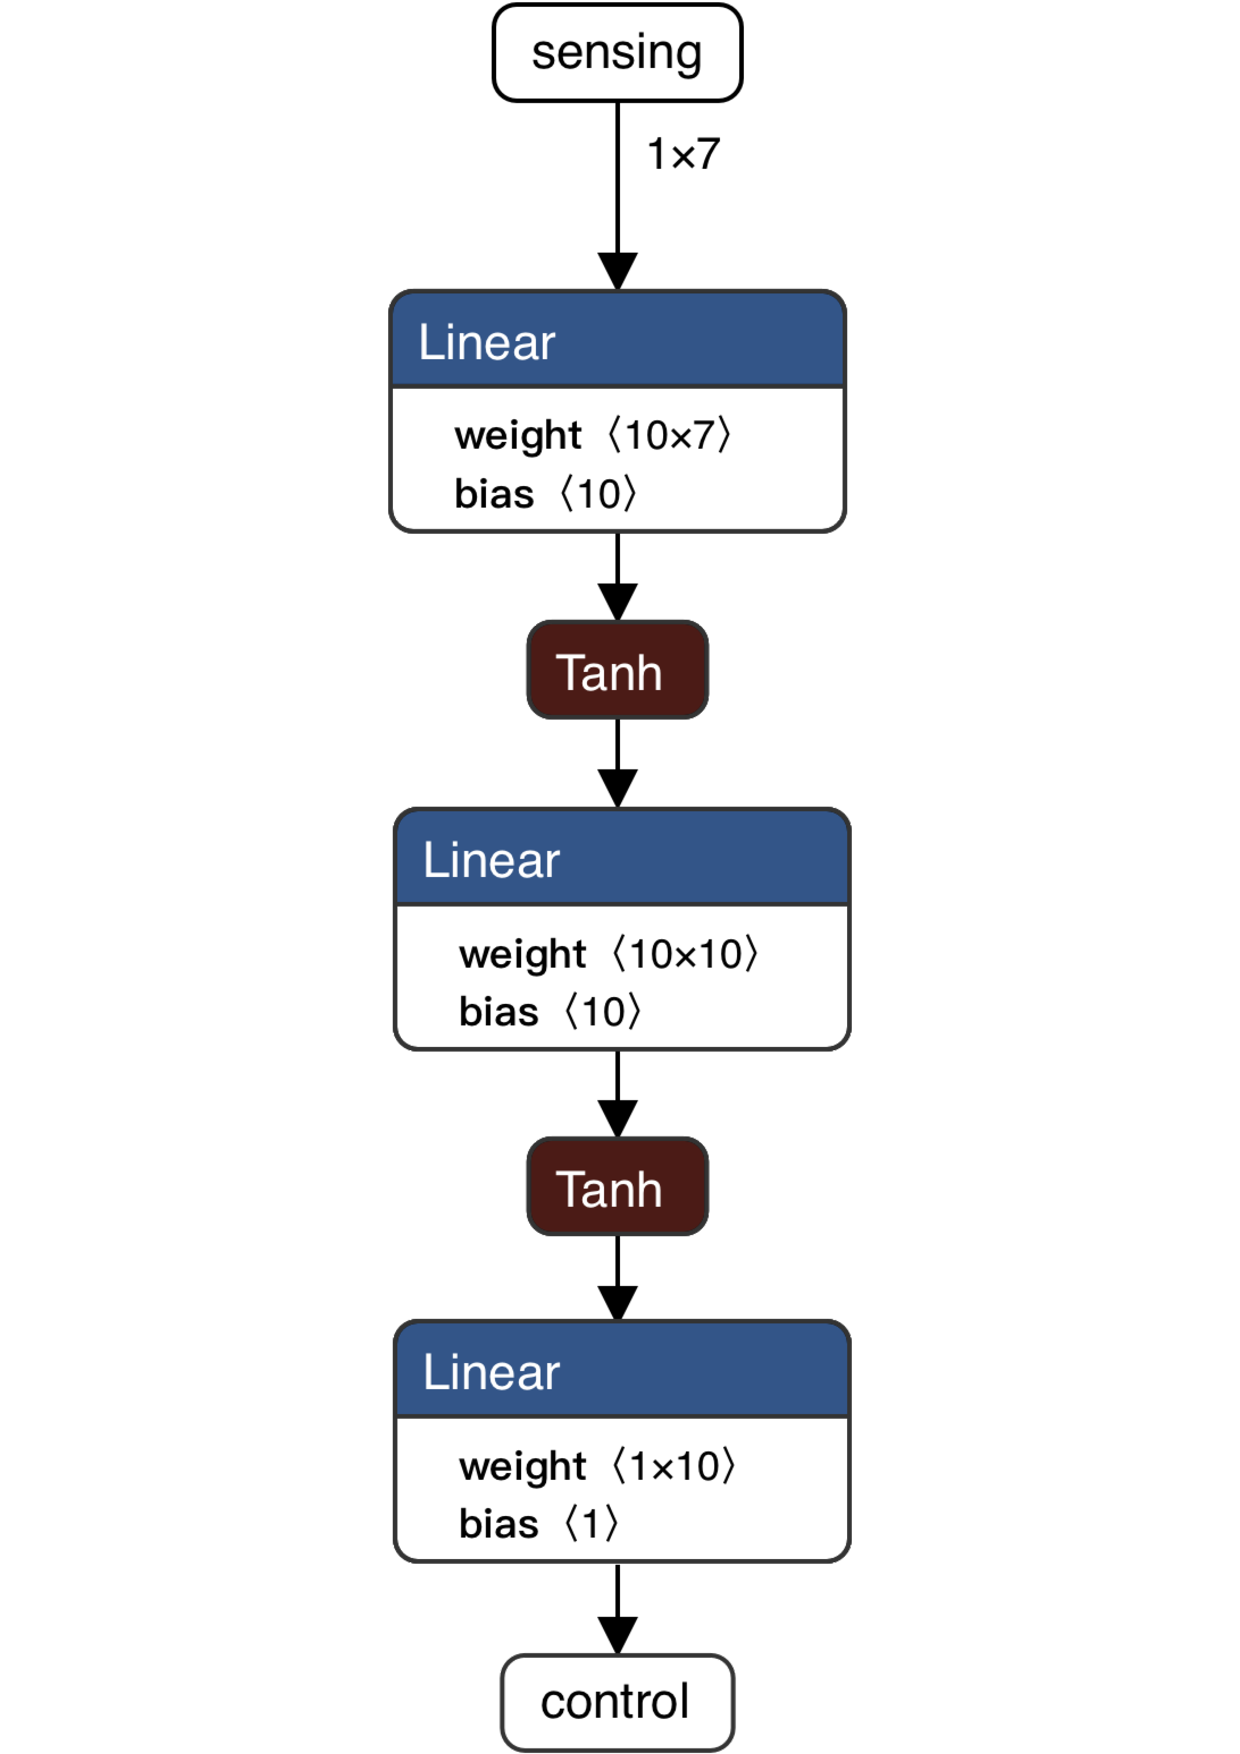
\includegraphics[width=.8\textwidth]{contents/images/task1distributed@4x}%
		\caption{Network with $7$ input sensing.}
		\label{fig:singlenet7distributed1}
	\end{subfigure}
	\hfill
	\begin{subfigure}[h]{0.495\textwidth}
		\centering
		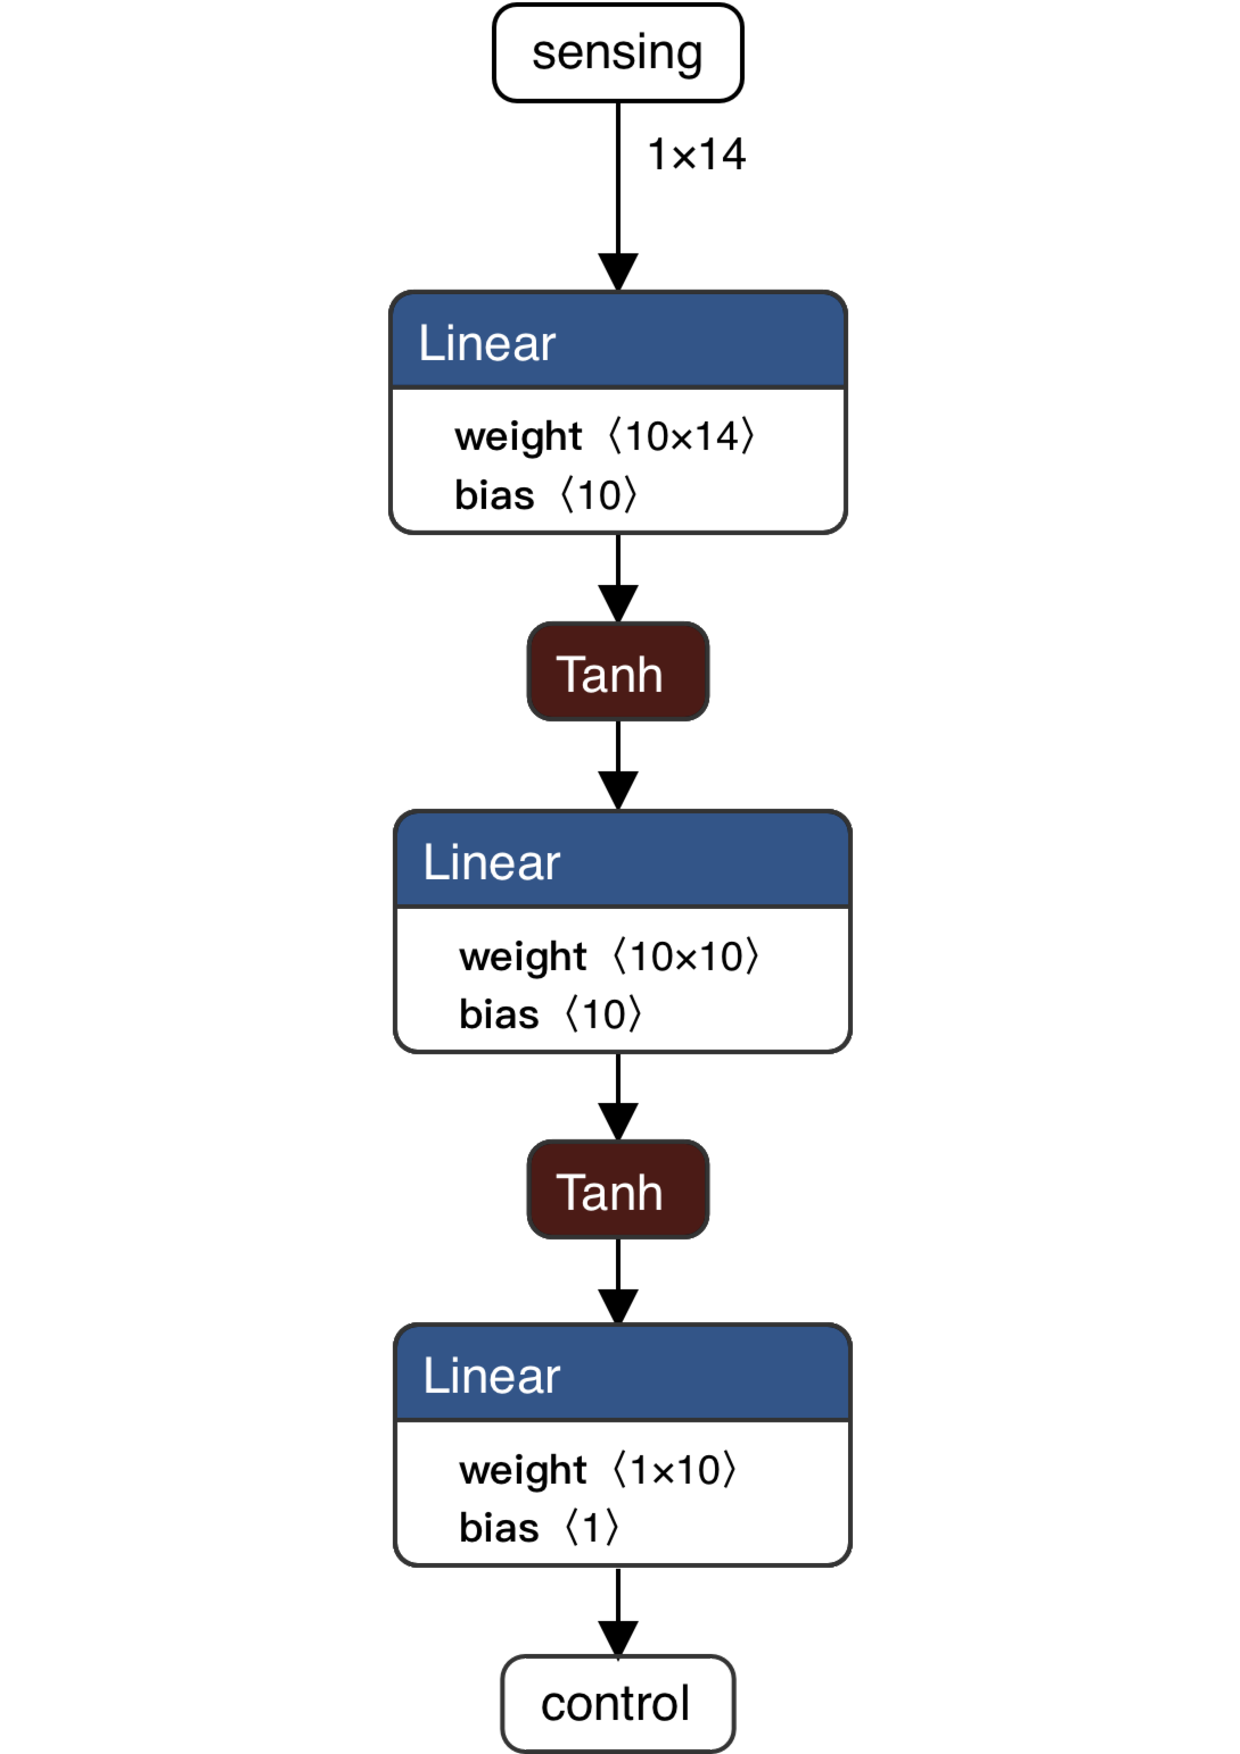
\includegraphics[width=.8\textwidth]{contents/images/task1distributed_all@4x}
		\caption{Network with $14$ input sensing.}
		\label{fig:singlenet14distributed1}
	\end{subfigure}
	\caption[Network architectures for the distributed approach.]{Visualisation of 
	the network architectures for the distributed approach.}
	\label{fig:singlenetdistributed1}
\end{figure}
To the first and second layer is applied a non-linear activation function, 
useful to make the model generalise. 
In particular, we chose the hyperbolic tangent (Tanh) 
\cite[see][]{kalman1992tanh}, a zero-centred function, shown in Figure 
\ref{fig:tanh}, whose range lies between $[-1, 1]$ and its output is given by

\begin{Equation}[H]
	\centering
	\begin{equation}
	f(x)= \frac{\sinh (x)}{\cosh (x)} = \bigg( \frac{e^x - e^{-x}}{e^x + 
		e^{-x}}\bigg)
	\end{equation}
	\caption{Hyperbolic Tangent Function (Tanh).}
	\label{eq:tanh}
\end{Equation}

This type of activation function is often used in deep learning and one of its 
advantages is that negative inputs are mapped to strongly negative values.

\begin{figure}[!htb]
	\centering
	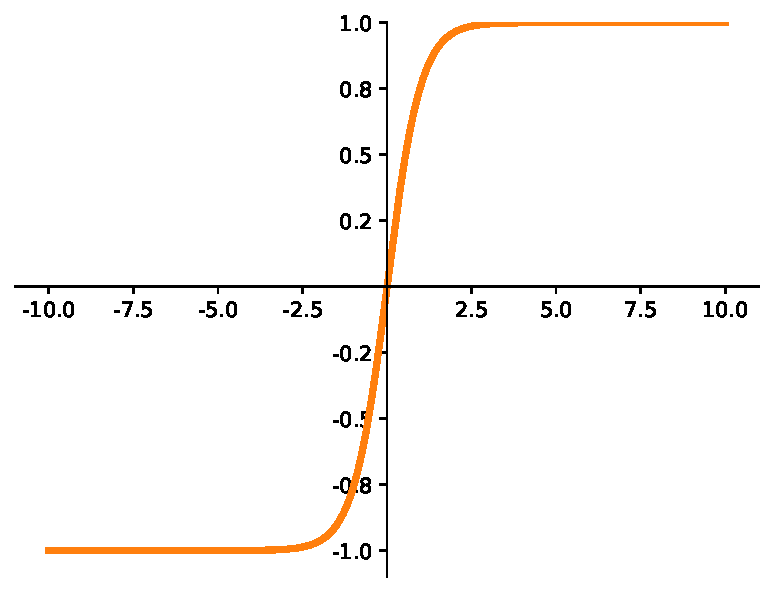
\includegraphics[width=.5\textwidth]{contents/images/tanh2}%
	\caption{Trend of the Tanh activation function.}
	\label{fig:tanh}
\end{figure}

%fixme citation
As optimiser, we chose Adam, {an algorithm for first-order gradient-based 
optimisation of stochastic objective functions, based on adaptive estimates of 
lower-order moments}, \cite[see][]{kingma2014adam, 
loshchilov2017decoupled}, 
implemented in the \texttt{torch.optim} package, with a learning rate of $0.01$. 

Instead of computing the gradient descent on the entire dataset, the training set is 
split in mini-batches of size $100$ and an approximation of the gradient is 
produced, which makes the algorithm faster and at the same time, for sufficiently 
large numbers, the result is indistinguishable.

Gradient descent algorithms are susceptible to ``get stuck'' in local minima.
Mini-batches shuffle facilitate to avoid this problem by enabling the gradient to 
``bounce'' out of eventual local minimum, making it more variable by exploiting 
randomness, thereby helping convergence.

All the models are trained for $50$ epochs and evaluated using the \gls{mse} loss 
function, often used in regression problems. 
This criterion, implemented in the \texttt{torch.nn} package, measures the 
average of squared error between predictions and targets and learns to reduce it 
by penalising big errors in the model predictions.

\begin{Equation}[!htb]
	\centering
	\begin{equation}
	\mathtt{MSE} = \frac{\sum_{i=1}^n (y_i-\hat y_i)^2}{n}
	\end{equation}
	\caption{Mean Squared Error (\gls{mse}) loss function.}
	\label{eq:mse}
\end{Equation}
	

\subsubsection{Experiments}
\label{subsubsec:expdist}

The first group of experiments carried out, summarised in Table 
\ref{tab:modeln5dist}, examines the behaviour of the control learned in the case 
of the three different inputs, \texttt{prox\_values}, \texttt{prox\_comm} or 
\texttt{all\_sensors}, for a number of robots $N$ and an \texttt{avg\_gap} both 
fixed respectively at $5$ and the second chosen between $8$, $13$ and $24$.
\begin{figure}[!htb]
	\centering
	\begin{tabular}{cccc}
		\toprule
		\textbf{Model} \quad & \textbf{\texttt{network\_input}} & 
		\textbf{\texttt{input\_size}} &
		\textbf{\texttt{avg\_gap}} \\
		\midrule
		\texttt{net1} 				 & \texttt{prox\_values}	&  $  7$  &  $  8$  \\
		\texttt{net2} 				& \texttt{prox\_values}	    &  $  7$  &  $13$ \\
		\texttt{net3} 				& \texttt{prox\_values}	    &  $  7$  &  $24$  \\
		\texttt{net4} 				 & \texttt{prox\_comm}	  &  $  7$  &  $  8$  \\
		\texttt{net5} 				 & \texttt{prox\_comm}	  &  $  7$  &  $13$  \\
		\texttt{net6} 				 & \texttt{prox\_comm}	  &  $  7$  &  $24$  \\
		\texttt{net7} 				 & \texttt{all\_sensors}	  &  $14$  &  $  8$  \\
		\texttt{net8} 				 & \texttt{all\_sensors}	  &  $14$  &  $13$ 	\\
		\texttt{net9} 				 & \texttt{all\_sensors}	  &  $14$  &  $24$ 	\\
		\bottomrule
	\end{tabular}
	\captionof{table}{List of the experiments carried out with $5$ agents.}
	\label{tab:modeln5dist}
\end{figure}

First of all we start by showing in Figure \ref{fig:distloss} an overview of the 
models performance in terms of train and validation losses. 
\begin{figure}[!htb]
	\centering
	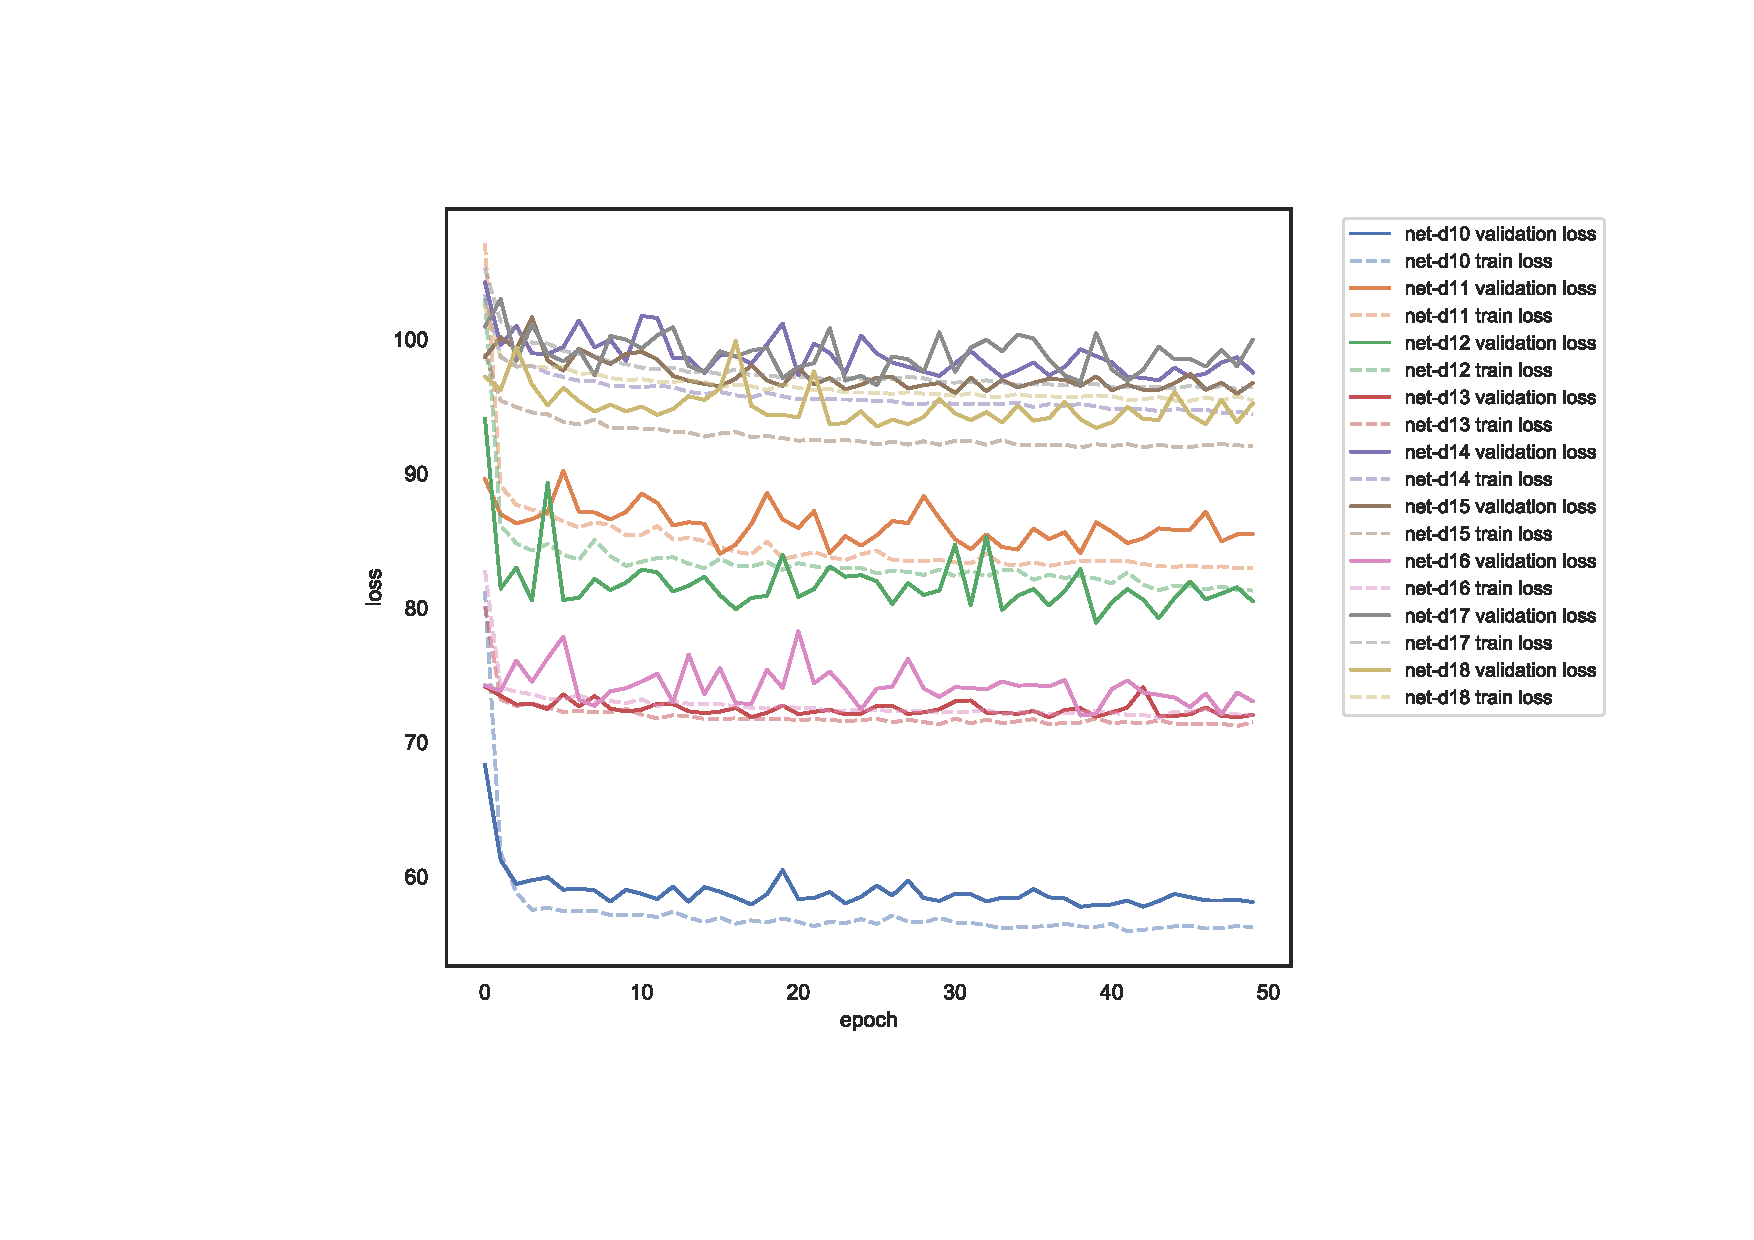
\includegraphics[width=.75\textwidth]{contents/images/task1/pdf/loss-distributed-all@}%
	\caption[Comparison of losses of the first set of 
	experiments.]{Comparison of 
	the losses of the models carried out with $5$ agents.}
	\label{fig:distloss}
\end{figure}
It is immediately evident that, in case of \texttt{prox\_values} inputs, the 
experiment performed with an \texttt{avg\_gap} of $24$ is not remarkable since 
this value exceeds the maximal range of the sensor.

We start the analysis by exploring the results of the experiments obtained 
using the \texttt{prox\_values} readings alone as input of the network, continuing 
the with \texttt{prox\_comm} and concluding with \texttt{all\_sensors}.
The performance of \texttt{net1} are shown in the following images. In particular,  
in Figure \ref{fig:net1r2} is visualised a comparison of the \gls{r2}, or coefficient 
of determination, of the manual and the learned controllers, on the validation set.
This score function evidences how well the regression predictions approximate 
the real data points (groundtruth). Since a model that perfectly predicts the data 
has a score of $1$, we assume that a higher score corresponds to a model that 
performs better.
\begin{figure}[!htb]
	\centering
	\begin{subfigure}[h]{0.49\textwidth}
		\centering
		\includegraphics[width=\textwidth]{contents/images/distr-net1/pdf/regression-manualvsomniscient}%
	\end{subfigure}
	\hfill
	\begin{subfigure}[h]{0.49\textwidth}
		\centering
		\includegraphics[width=\textwidth]{contents/images/distr-net1/pdf/regression-net1-vs-omniscient}
	\end{subfigure}
	\caption[Evaluation of the \gls{r2} coefficients of \texttt{net1} 
	.]{Comparison of 
	the \gls{r2} coefficient of the manual and the controller learned from 
	\texttt{net1} with respect to the omniscient one.}
	\label{fig:net1r2}
\end{figure}
From these figures we expect that the robots' behaviour using the learned 
controller instead of the manual one is a bit better, even if far from the omniscient 
controller.

In Figure \ref{fig:net1traj} we show first a comparison of the expert and the 
learned trajectories, and then between the manual and the learned ones. In 
particular, on the y-axis is visualised the position of each agent over time, while 
on the x-axis the simulation timesteps. It is important to notice that the plots 
summarise all the runs: at each timestep, the position of each agent is presented 
as an average over all the simulation runs, and besides is  shown this average 
minus and plus the standard deviation.
\begin{figure}[!htb]
	\centering
	\begin{subfigure}[h]{0.49\textwidth}
		\centering
		\includegraphics[width=\textwidth]{contents/images/distr-net1/pdf/position-overtime-omniscient}%
		\caption{Expert controller trajectories.}
	\end{subfigure}
	\hfill
	\begin{subfigure}[h]{0.49\textwidth}
		\centering
		\includegraphics[width=\textwidth]{contents/images/distr-net1/pdf/position-overtime-distributed}
		\caption{Distributed controller trajectories.}
	\end{subfigure}
	\hspace*{\fill}%          % empty line absolutely necessary!
	
	\vspace*{8pt}%  
	
	\hspace*{\fill}%  
	\begin{subfigure}[h]{0.49\textwidth}
		\centering
		\includegraphics[width=\textwidth]{contents/images/distr-net1/pdf/position-overtime-manual}%
		\caption{Manual controller trajectories.}
	\end{subfigure}
	\hfill
	\begin{subfigure}[h]{0.49\textwidth}
		\centering
		\includegraphics[width=\textwidth]{contents/images/distr-net1/pdf/position-overtime-distributed}
		\caption{Distributed controller trajectories.}
	\end{subfigure}
	\caption[Evaluation of the trajectories learned by \texttt{net1}.]{Comparison 
		of trajectories generated using three controllers: the expert, the manual and 
		the one learned from \texttt{net1}.}
	\label{fig:net1traj}
\end{figure}

The convergence of the robots to the target using the omniscient controller is 
much faster than that with the manual or the learned one. In particular, the 
learned trajectories, even if converge to the correct configuration they require a 
higher number of timesteps, sometimes even 40 timesteps may be necessary, 
compared to the two others controllers, where less than 10 timesteps are 
sufficient.

\begin{figure}[!htb]
	\centering
	\begin{subfigure}[h]{0.3\textwidth}
		\centering
		\includegraphics[width=\textwidth]{contents/images/distr-net1/pdf/control-overtime-omniscient}%
		\caption{Expert controller.}
	\end{subfigure}
	\hfill
	\begin{subfigure}[h]{0.3\textwidth}
		\centering
		\includegraphics[width=\textwidth]{contents/images/distr-net1/pdf/control-overtime-manual}%
		\caption{Manual controller.}
	\end{subfigure}
	\hfill
	\begin{subfigure}[h]{0.3\textwidth}
		\centering
		\includegraphics[width=\textwidth]{contents/images/distr-net1/pdf/control-overtime-distributed}
		\caption{Distributed controller.}
	\end{subfigure}
	\caption[Evaluation of the control learned by \texttt{net1}.]{Comparison 
		of output control generated using three controllers: the expert, the manual 
		and the one learned from \texttt{net1}.}
	\label{fig:net1control}
\end{figure}

In fact, analysing in Figure \ref{fig:net1control} the evolution of the control over 
time, it is possible to notice that the omniscient in the first timesteps uses a 
higher speed than that chosen by the manual controller or the one predicted by 
the network. After about $10$ timesteps they both reach the target, with a 
certain tolerance, maintaining then the speed constant at $0$. Instead, the 
distributed controller decreases the speed of the agents as the timesteps pass, 
reaching zero speed but with a certain variance.

A couple of useful plots are shown below. In Figure \ref{fig:net1responsesensors} 
is visualised the response of the learned controller as the input sensing changes. 
\begin{figure}[!htb]
	\centering
	\begin{subfigure}[h]{0.49\textwidth}
		\centering
		\includegraphics[width=\textwidth]{contents/images/distr-net1/pdf/response-net1-front}%
		%\caption{response-net1-net([0, 0, x, 0, 0, 0, 0]).}
	\end{subfigure}
	\hfill
	\begin{subfigure}[h]{0.49\textwidth}
		\centering
		\includegraphics[width=\textwidth]{contents/images/distr-net1/pdf/response-net1-rear}
		%\caption{response-net1-net([0, 0, 0, 0, 0, x, x]).}
	\end{subfigure}
	\caption[Response of \texttt{net1} by varying the input sensing.]{Response of 
		\texttt{net1} by varying the input sensing.}
	\label{fig:net1responsesensors}
\end{figure}

In particular we analyse two cases. The first one shows the control predicted by 
the network when the robot sees nothing behind but only in front, more 
specifically when the given input is  $([0, 0, x, 0, 0, 0, 0])$, with $x$ varying in the 
range $[0, 4500]$.
The second shows the control predicted by the network when the robot instead 
sees nothing in front but only behind, more specifically when the given input is  
$([0, 0, 0, 0, 0,x , x])$, with $x$ varying in the range $[0, 4500]$.

The behaviour is almost as expected. When the robot sees nothing behind but 
something in front, the model returns a negative speed, since the robot has to 
move backwards. 
The absolute value of control increases as the proximity to the obstacle increases.
The same behaviour is obtained when the robot sees only behind but nothing in 
front. In this case the speed has the opposite sign.

In Figure \ref{fig:net1responseposition} another informative plot displays the 
behaviour of a robot located between two that are already in their place.
It visualises the response of the learned controller by varying the distance 
between two stationary agents and a robot located halfway between them.
On the x-axis is visualised the position of the moving robot, while on the y-axis 
the output control, computed as an average over $100$ measures in which the 
pose of the agent $(x, y, \theta)$ differs by a certain epsilon uniformly distributed 
in the range $[-0.5, 0.5]$. In this way, the result obtained avoids the effects of 
noise that would be obtained on a single measurement and unrealistic artefacts in 
which the sensors are not continuous, compared to the pose, in simulation. In 
addition are also shown the bands that represent plus and minus standard 
deviation.
\begin{figure}[!htb]
	\centering
	\includegraphics[width=.75\textwidth]{contents/images/distr-net1/pdf/response-varying_init_position-net1}%
	\caption{Response of \texttt{net1} by varying the initial position.}
	\label{fig:net1responseposition}
\end{figure}

As expected, the output is a high positive value when the robot is close to an 
obstacle on the left, it decreases and reaches $0$ when the distance from right 
and left is equal, and finally becomes negative when there is an obstacle in front 
and not behind.

Finally, in Figure \ref{fig:net1distance} is presented another useful metric that 
measures the absolute distance of each robot from the target, visualised on the 
y-axis, over time. This value is averaged on all robots among all the simulation 
runs. The median value is shown as well as the interquartile and interdecile ranges.
\begin{figure}[!htb]
	\centering
	\includegraphics[width=.75\textwidth]{contents/images/distr-net1/pdf/distances-from-goal-compressed-distributed}%
	\caption[Evaluation of \texttt{net1} distances from goal.]{Comparison of 
	performance in terms of distances from goal obtained using three controllers: 
	the expert, the manual and the one learned from \texttt{net1}.}
	\label{fig:net1distance}
\end{figure}

On average, the distance from goal of the learned controller is lower than the one 
obtained with the manual controller, that means that in the final configuration 
the robots moved following the learned controller are closer to the target than 
those moved with the manual one, which are on average at a distance of about 
$1$ \gls{cm} from the goal position. 

As mentioned before, in case of \texttt{prox\_values} inputs the 
experiment performed with an \texttt{avg\_gap} of $24$ is not meaningful since 
this value exceeds the maximal range of the sensor. Similarly, since $14$ is the 
maximum range, it is difficult to use this type of input when the \texttt{avg\_gap}  
is $13$, as shown by the losses in Figure \ref{fig:distlossprox_values}.
\begin{figure}[!htb]
	\centering
	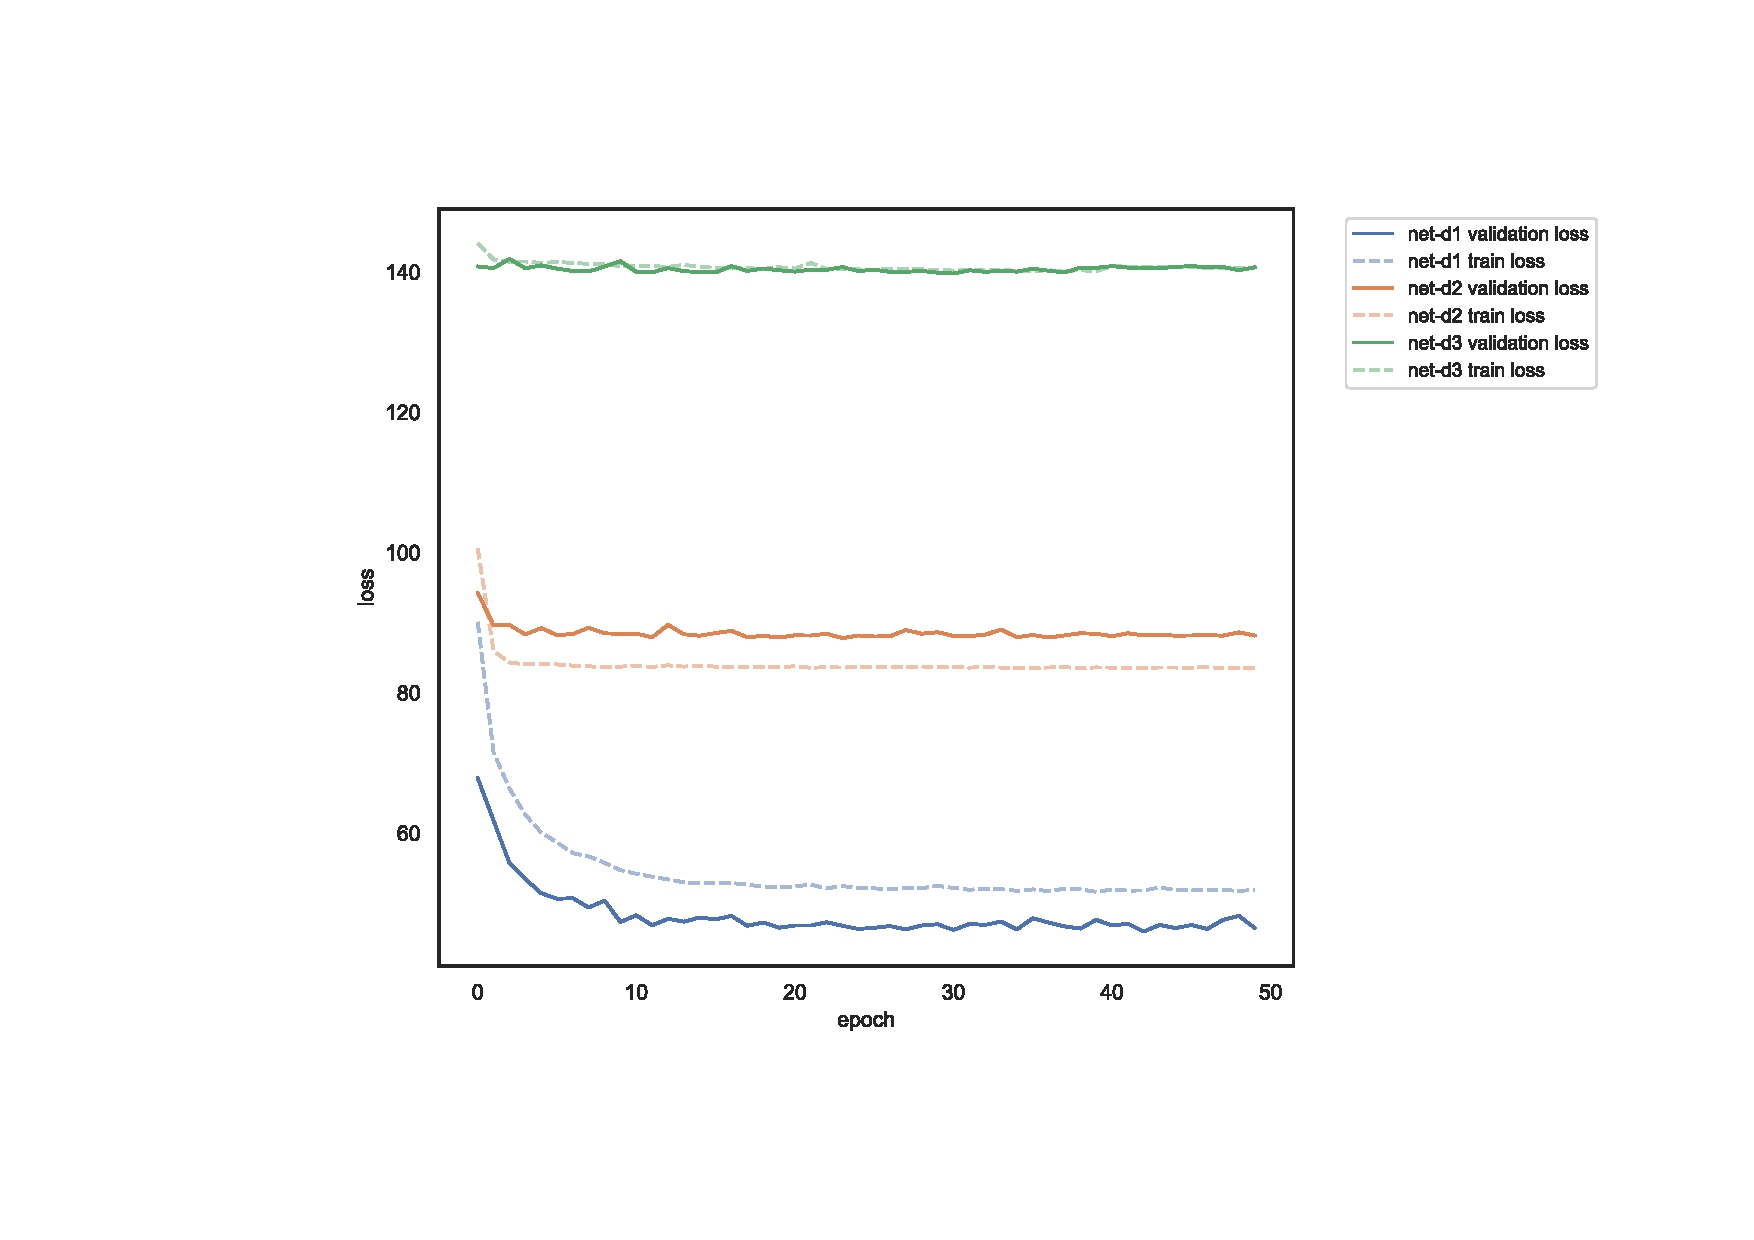
\includegraphics[width=.7\textwidth]{contents/images/task1/pdf/loss-distributed-prox_values@}%
	\caption{Comparison of the losses of the models that use \texttt{prox\_values} 
		readings.}
	\label{fig:distlossprox_values}
\end{figure}

Following are shown the results of the experiments obtained using the 
\texttt{prox\_comm} readings. In Figure \ref{fig:distlossprox_comm}, are 
analysed the losses by varying the average gap. From a first observation the 
network seems to be able to work with all the gaps.
\begin{figure}[!htb]
	\centering
	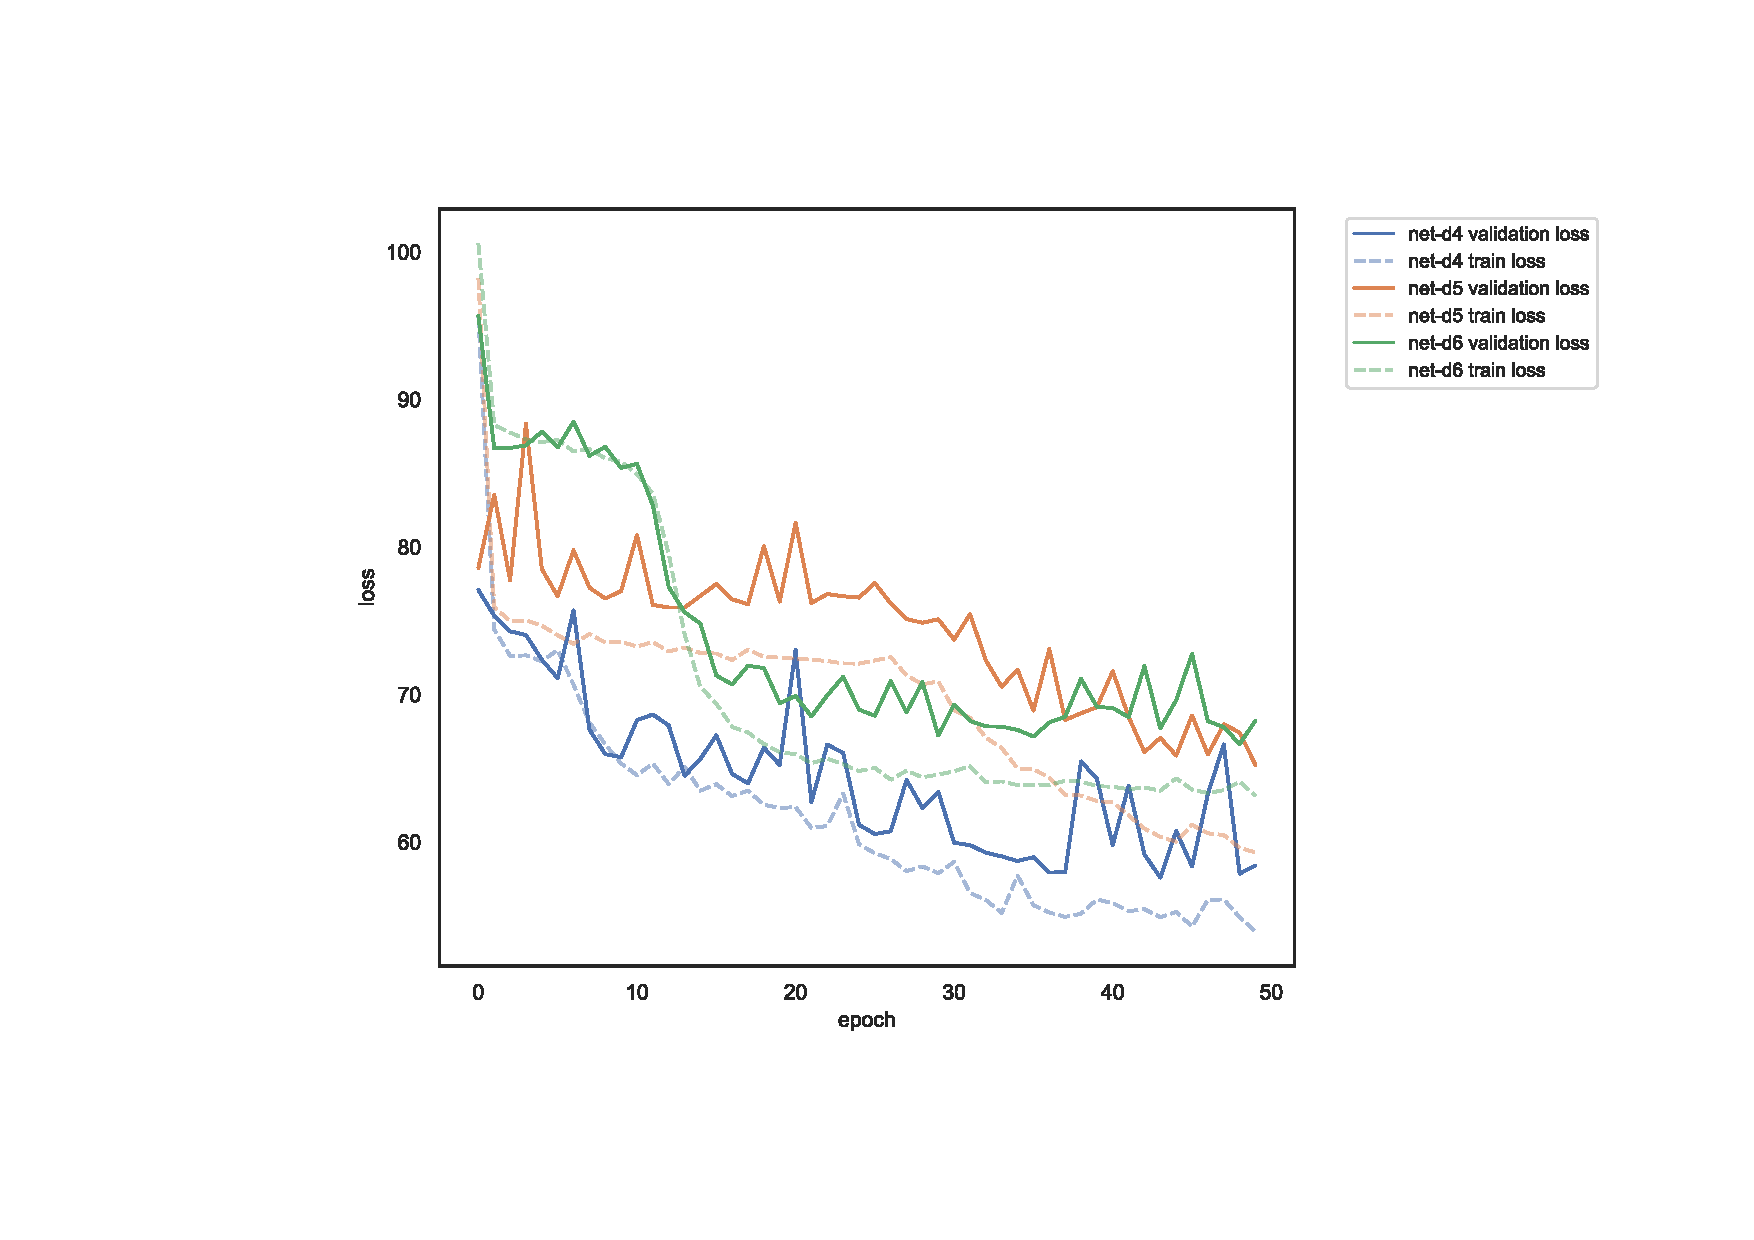
\includegraphics[width=.7\textwidth]{contents/images/task1/pdf/loss-distributed-prox_comm@}%
	\caption{Comparison of the losses of the models that use \texttt{prox\_comm} 
	readings.}
	\label{fig:distlossprox_comm}
\end{figure}

Then we move on to examine the \gls{r2} coefficients, visualised in Figure 
\ref{fig:net456r2}.
\begin{figure}[!htb]
	\begin{center}
		\begin{subfigure}[h]{0.47\textwidth}
			\includegraphics[width=\textwidth]{contents/images/distr-net4/pdf/regression-net4-vs-omniscient}%
		\end{subfigure}
		\hfill
		\begin{subfigure}[h]{0.47\textwidth}
			\includegraphics[width=\textwidth]{contents/images/distr-net5/pdf/regression-net5-vs-omniscient}%
		\end{subfigure}
	\end{center}
	\begin{center}
		\begin{subfigure}[h]{0.47\textwidth}
			\includegraphics[width=\textwidth]{contents/images/distr-net6/pdf/regression-net6-vs-omniscient}
		\end{subfigure}
	\end{center}
	\caption[Comparison of the \gls{r2} coefficients for \texttt{prox\_comm} 
	readings.]{Comparison of the \gls{r2} coefficients of the models that use 
	\texttt{prox\_comm} readings.}
	\label{fig:net456r2}
\end{figure}

The coefficient obtained with \texttt{net6} is higher than the others. For the 
assumptions made before we believe that the behaviour of this model is more 
promising. Moreover, as shown in Figure \ref{fig:net6r2}, we expect that the 
robots’ behaviour using the learned controller instead of the manual one is 
better, even if still far from the expert.

\begin{figure}[!htb]
	\centering
	\begin{subfigure}[h]{0.49\textwidth}
		\centering
		\includegraphics[width=\textwidth]{contents/images/distr-net6/pdf/regression-manualvsomniscient}%
	\end{subfigure}
	\hfill
	\begin{subfigure}[h]{0.49\textwidth}
		\centering
		\includegraphics[width=\textwidth]{contents/images/distr-net6/pdf/regression-net6-vs-omniscient}
	\end{subfigure}
	\caption[Evaluation of the \gls{r2} coefficients of \texttt{net6} 
	.]{Comparison of 
	the \gls{r2} coefficient of the manual and the controller 
	learned from \texttt{net6} with respect to the omniscient one.}
	\label{fig:net6r2}
\end{figure}

In Figure \ref{fig:net6traj} are shown the trajectories obtained employing the 
three controllers. 
As before, the robot positions are averaged over all the runs. 
Even for the expert, the convergence to the target is slower than before, 
as expected since the distance between the robots is greater, but it is much faster 
than with the other two controllers.
The manual controller has serious problems in reaching the goal: even if the 
\begin{figure}[!htb]
	\begin{center}
		\begin{subfigure}[h]{0.49\textwidth}
			\centering
			\includegraphics[width=\textwidth]{contents/images/distr-net6/pdf/position-overtime-omniscient}%
			\caption{Expert controller trajectories.}
		\end{subfigure}
		\hfill
		\begin{subfigure}[h]{0.49\textwidth}
			\centering
			\includegraphics[width=\textwidth]{contents/images/distr-net6/pdf/position-overtime-distributed}
			\caption{Distributed controller trajectories.}
		\end{subfigure}
	\end{center}
	\caption[Evaluation of the trajectories learned by 
	\texttt{net6}.]{Comparison of trajectories generated using three 
		controllers: the expert, the manual and the one learned from \texttt{net6}.}
\end{figure}
\medskip
\begin{figure}[!htb]\ContinuedFloat
	\centering
	\begin{subfigure}[h]{0.49\textwidth}
		\centering			
		\includegraphics[width=\textwidth]{contents/images/distr-net6/pdf/position-overtime-manual}%
		\caption{Manual controller trajectories.}
	\end{subfigure}
	\hfill
	\begin{subfigure}[h]{0.49\textwidth}
		\centering
		\includegraphics[width=\textwidth]{contents/images/distr-net6/pdf/position-overtime-distributed}
		\caption{Distributed controller trajectories.}
	\end{subfigure}
	\caption[]{Comparison 
		of trajectories generated using three controllers: the expert, the manual 
		and the one learned from \texttt{net6} (cont.).}
	\label{fig:net6traj}
\end{figure}
\noindent
agents try to position themselves at equal distances, they tend to increase the 
average gap between them, creating situations in which the last robot in motion 
hits the fixed one. Surprisingly, the learned controller allows the agents to 
converge to the correct configuration by taking more time than the expert does.

\begin{figure}[!htb]
	\centering
	\begin{subfigure}[h]{0.3\textwidth}
		\centering
		\includegraphics[width=\textwidth]{contents/images/distr-net6/pdf/control-overtime-omniscient}%
		\caption{Expert controller.}
	\end{subfigure}
	\hfill
	\begin{subfigure}[h]{0.3\textwidth}
		\centering
		\includegraphics[width=\textwidth]{contents/images/distr-net6/pdf/control-overtime-manual}%
		\caption{Manual controller.}
	\end{subfigure}
	\hfill
	\begin{subfigure}[h]{0.3\textwidth}
		\centering
		\includegraphics[width=\textwidth]{contents/images/distr-net6/pdf/control-overtime-distributed}
		\caption{Distributed controller.}
	\end{subfigure}
	\caption[Evaluation of the control learned by \texttt{net6}.]{Comparison 
		of output control generated using three controllers: the expert, the manual 
		and the one learned from \texttt{net6}.}
	\label{fig:net6control}
\end{figure}

As before, an immediate examination of the evolution of the control over 
time, in Figure \ref{fig:net6control}, highlights the speed of the expert 
controller, which in all the simulation runs after $25$ timesteps has reached the 
goal. 
In addition, the manual controller always sets a positive speed, which leads to the 
wrong behaviour mentioned earlier, while the slowness of the distributed 
control is explained by the use of a low speed.

Figure \ref{fig:net6responsesensors} visualises the response of the learned 
controller as the input sensing changes, analysing the same two cases as before. 
Despite the behaviour is the same obtained using \texttt{prox\_values} when the 
robot sees only behind, this time the trend is different when the robot sees 
nothing behind: since the robot has to move backwards, a negative speed is 
always returned, that is higher when the obstacle is far. 
\begin{figure}[!htb]
	\centering
	\begin{subfigure}[h]{0.49\textwidth}
		\centering
		\includegraphics[width=\textwidth]{contents/images/distr-net6/pdf/response-net6-front}%
	\end{subfigure}
	\hfill
	\begin{subfigure}[h]{0.49\textwidth}
		\centering
		\includegraphics[width=\textwidth]{contents/images/distr-net6/pdf/response-net6-rear}
	\end{subfigure}
	\caption{Response of \texttt{net6} by varying the input sensing.}
	\label{fig:net6responsesensors}
\end{figure}

In Figure \ref{fig:net6responseposition} is displayed the behaviour of a robot 
located between two that are already in their place.
\begin{figure}[!htb]
	\centering
	\includegraphics[width=.75\textwidth]{contents/images/distr-net6/pdf/response-varying_init_position-net6}%
	\caption{Response of \texttt{net6} by varying the initial position.}
	\label{fig:net6responseposition}
\end{figure}
It visualises the response of the learned controller by varying the distance 
between two stationary agents and a robot located among them.
As expected, the output is a high positive value when the robot is close to an 
obstacle on the left, it decreases and reaches $0$ when the distance from 
right and left is equal, and finally becomes negative when there is an obstacle in 
front and not behind. 

Finally, in Figure \ref{fig:net6distance} is presented the average distance of the 
robots from the target among all the simulations. 
\begin{figure}[!htb]
	\centering
	\includegraphics[width=.75\textwidth]{contents/images/distr-net6/pdf/distances-from-goal-compressed-distributed}%
		\caption[Evaluation of \texttt{net6} distances from goal.]{Comparison of 
		performance in terms of distances from goal obtained using three 
		controllers: the expert, the manual and the one learned from \texttt{net6}.}
	\label{fig:net6distance}
\end{figure}
The performance of the learned and the manual controllers are similar: in the 
final configuration they both are at about $5$ \gls{cm} from the target. 

We conclude the first group of experiments presenting the results obtained 
using both types of input together from which we expect a more stable and 
robust behaviour. 

In Figure \ref{fig:distlossall}, are analysed the losses by varying the average gap. 
\begin{figure}[!htb]
	\centering
	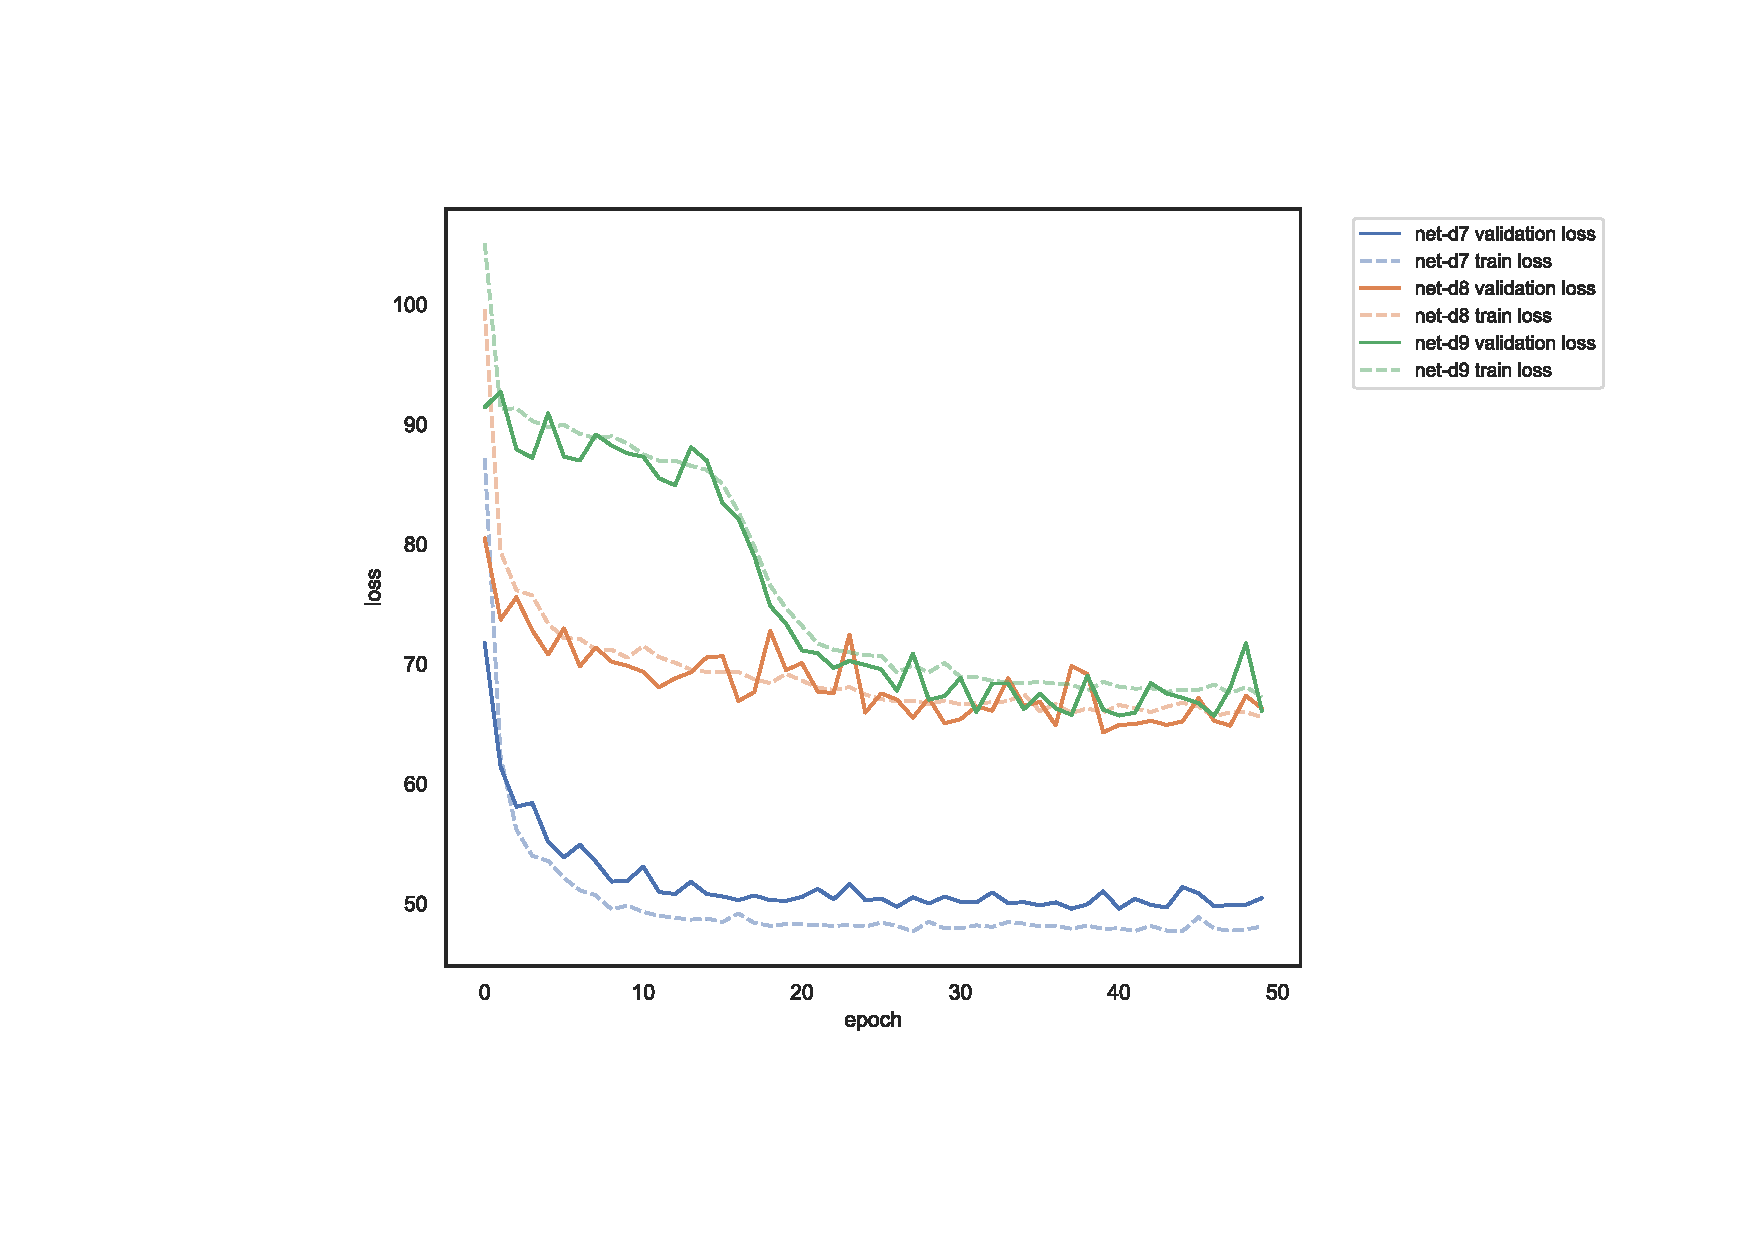
\includegraphics[width=.7\textwidth]{contents/images/task1/pdf/loss-distributed-all_sensors@}%
	\caption{Comparison of the losses of the models that use \texttt{all\_sensors} 
		readings.}
	\label{fig:distlossall}
\end{figure}
Using \texttt{all\_sensors} inputs the network is able to work well with all the 
gaps. 

Examining the \gls{r2} coefficients in Figure \ref{fig:net789r2}, the behaviour 
obtained with \texttt{net7} and \texttt{net9} are the more promising. 
\begin{figure}[!htb]
	\begin{center}
		\begin{subfigure}[h]{0.49\textwidth}
 			\includegraphics[width=\textwidth]{contents/images/distr-net7/pdf/regression-net7-vs-omniscient}%
		\end{subfigure}
		\hfill
		\begin{subfigure}[h]{0.49\textwidth}
			\includegraphics[width=\textwidth]{contents/images/distr-net8/pdf/regression-net8-vs-omniscient}%
		\end{subfigure}
	\end{center}
	\begin{center}
		\begin{subfigure}[h]{0.49\textwidth}
			\includegraphics[width=\textwidth]{contents/images/distr-net9/pdf/regression-net9-vs-omniscient}
		\end{subfigure}
	\end{center}
	\caption[Comparison of the \gls{r2} coefficients for \texttt{prox\_comm} 
	readings.]{Comparison of the \gls{r2} coefficients of the models that use 
		\texttt{prox\_comm} readings.}
	\label{fig:net789r2}
\end{figure}

This is further supported by the comparisons in Figures \ref{fig:net7r2} and 
\ref{fig:net9r2}, which prove the superiority of these controllers.
\begin{figure}[!htb]
	\centering
	\begin{subfigure}[h]{0.49\textwidth}
		\centering
		\includegraphics[width=\textwidth]{contents/images/distr-net7/pdf/regression-manualvsomniscient}%
	\end{subfigure}
	\hfill
	\begin{subfigure}[h]{0.49\textwidth}
		\centering
		\includegraphics[width=\textwidth]{contents/images/distr-net7/pdf/regression-net7-vs-omniscient}
	\end{subfigure}
	\caption[Evaluation of the \gls{r2} coefficients of \texttt{net7} 
	.]{Comparison of 
		the \gls{r2} coefficient of the manual and the controller 
		learned from \texttt{net7} with respect to the omniscient one.}
	\label{fig:net7r2}
\end{figure}
\begin{figure}[!htb]
	\centering
	\begin{subfigure}[h]{0.49\textwidth}
		\centering
		\includegraphics[width=\textwidth]{contents/images/distr-net9/pdf/regression-manualvsomniscient}%
	\end{subfigure}
	\hfill
	\begin{subfigure}[h]{0.49\textwidth}
		\centering
		\includegraphics[width=\textwidth]{contents/images/distr-net9/pdf/regression-net9-vs-omniscient}
	\end{subfigure}
	\caption[Evaluation of the \gls{r2} coefficients of \texttt{net9} 
	.]{Comparison of 
		the \gls{r2} coefficient of the manual and the controller 
		learned from \texttt{net9} with respect to the omniscient one.}
	\label{fig:net9r2}
\end{figure}

Taking into consideration once again the more complex case, that is the one 
with the greatest average gap, we show in Figure \ref{fig:net9traj} trajectories 
obtained employing the three controllers. 

The convergence to the target is still slow, even if this time the expert need 
less timesteps than before.The manual controller does not shows the same 
problem has before, while the learned controller is still the slowest to end up in 
the correct configuration.
\begin{figure}[!htb]
	\begin{center}
		\begin{subfigure}[h]{0.49\textwidth}
			\centering
			\includegraphics[width=\textwidth]{contents/images/distr-net9/pdf/position-overtime-omniscient}%
			\caption{Expert controller trajectories.}
		\end{subfigure}
		\hfill
		\begin{subfigure}[h]{0.49\textwidth}
			\centering
			\includegraphics[width=\textwidth]{contents/images/distr-net9/pdf/position-overtime-distributed}
			\caption{Distributed controller trajectories.}
		\end{subfigure}
	\end{center}
	\caption[Evaluation of the trajectories learned by 
	\texttt{net9}.]{Comparison of trajectories generated using three controllers: the 
	expert, the manual and the one learned from \texttt{net9}.}
\end{figure}
\medskip
\begin{figure}[!htb]\ContinuedFloat
	\centering
	\begin{subfigure}[h]{0.49\textwidth}
		\centering
		\includegraphics[width=\textwidth]{contents/images/distr-net9/pdf/position-overtime-manual}%
		\caption{Manual controller trajectories.}
	\end{subfigure}
	\hfill
	\begin{subfigure}[h]{0.49\textwidth}
		\centering
		\includegraphics[width=\textwidth]{contents/images/distr-net9/pdf/position-overtime-distributed}
		\caption{Distributed controller trajectories.}
	\end{subfigure}
	\caption[]{Comparison of trajectories generated using three controllers: the 
	expert, the manual and the one learned from \texttt{net9} (cont.).}
	\label{fig:net9traj}
\end{figure}

Examining the evolution of the output control, in Figure \ref{fig:net9control}, 
the plots of the expert and the learned controller are similar, although the speed 
in the second is much lower.
\begin{figure}[!htb]
	\centering
	\begin{subfigure}[h]{0.3\textwidth}
		\centering
		\includegraphics[width=\textwidth]{contents/images/distr-net9/pdf/control-overtime-omniscient}%
		\caption{Expert controller.}
	\end{subfigure}
	\hfill
	\begin{subfigure}[h]{0.3\textwidth}
		\centering
		\includegraphics[width=\textwidth]{contents/images/distr-net9/pdf/control-overtime-manual}%
		\caption{Manual controller.}
	\end{subfigure}
	\hfill
	\begin{subfigure}[h]{0.3\textwidth}
		\centering
		\includegraphics[width=\textwidth]{contents/images/distr-net9/pdf/control-overtime-distributed}
		\caption{Distributed controller.}
	\end{subfigure}
	\caption[Evaluation of the control learned by \texttt{net9}.]{Comparison 
		of output control generated using three controllers: the expert, the manual 
		and the one learned from \texttt{net9}.}
	\label{fig:net9control}
\end{figure}

In Figure \ref{fig:net9responseposition} is displayed the behaviour of a robot 
located between two that are already in their place.
\begin{figure}[!htb]
	\centering
	%FIXME change image and put .75 
	\includegraphics[width=.75\textwidth]{contents/images/distr-net9/pdf/response-varying_init_position-net9}%
	\caption{Response of \texttt{net9} by varying the initial position.}
	\label{fig:net9responseposition}
\end{figure}
This time the trend of the three curves shows how the behaviour of the model 
learned and of the manual controller are similar to that of the expert.

Finally, in Figure \ref{fig:net9distance} is presented the absolute distance of each 
robot from the target, averaged on all robots among all the simulation runs. The 
median value is shown as well as the interquartile and interdecile ranges.
\begin{figure}[!htb]
	\centering
	\includegraphics[width=.75\textwidth]{contents/images/distr-net9/pdf/distances-from-goal-compressed-distributed}%
	\caption[Evaluation of \texttt{net9} distances from goal.]{Comparison of 
		performance in terms of distances from goal obtained using three 
		controllers: the expert, the manual and the one learned from \texttt{net9}.}
	\label{fig:net9distance}
\end{figure}

As anticipated by the trajectories in Figure \ref{fig:net9traj}, the controller 
learned from \texttt{net9} is slower to converge than the manual one. In fact, 
this plot confirms that the agents moved following a manual controller in the final 
configuration are closer to the target than those moved by the distributed 
controller, respectively, they are on average $2$ or $6$ \gls{cm} away from the 
goal position.

To summarise the performance, as the different inputs of the network vary,for 
each gap, we show once again in the figures below the losses of the trained 
models.

In case of an \texttt{avg\_gap} of $8$ \gls{cm}, the model trained using 
\texttt{prox\_values} as input has a lower loss, following is the network that 
employ \texttt{all\_sensors}, with a very similar value, and at the end the model 
that works with \texttt{prox\_comm}.
\begin{figure}[!htb]
	\centering
	\includegraphics[width=.7\textwidth]{contents/images/task1/pdf/loss-distributed-avg8@}%
	\caption{Comparison of the losses of the models that use an \texttt{avg\_gap} 
		of $8$ \gls{cm}.}
	\label{fig:distloss8}
\end{figure}
It is quite obvious that the performance obtained using as inputs 
\texttt{prox\_values} and \texttt{all\_sensors} are the best, as well as the fact that 
\texttt{all\_sensors} cannot perform better than the other since using also the 
data coming from \texttt{prox\_comm}, that is not able to work well with small 
gaps, contains in the second half of the array unusable values.

\begin{figure}[!htb]
	\centering
	\includegraphics[width=.7\textwidth]{contents/images/task1/pdf/loss-distributed-avg13@}%
	\caption{Comparison of the losses of the models that use an \texttt{avg\_gap} 
		of $13$ \gls{cm}.}
	\label{fig:distloss13}
\end{figure}
In a complementary way, by increasing the gap to $13$ \gls{cm},  
\texttt{prox\_values} alone is not able to achieve satisfactory results, while used 
together with \texttt{prox\_comm}, \texttt{all\_sensors} reaches good 
performances that on the validation set are comparable to those obtained using 
\texttt{prox\_comm} alone.

Finally, by increasing the gap even more, up to $24$ \gls{cm}, 
\texttt{prox\_values} becomes completely unusable, while \texttt{prox\_comm} 
and \texttt{all\_sensors} still have excellent performances.
\begin{figure}[!htb]
	\centering
	\includegraphics[width=.7\textwidth]{contents/images/task1/pdf/loss-distributed-avg24@}%
	\caption{Comparison of the losses of the models that use an \texttt{avg\_gap} 
	of $24$ \gls{cm}.}
	\label{fig:distloss24}
\end{figure}

The last group of experiments we carried out using a distributed approach, 
examines the behaviour of the control learned just in case of \texttt{all\_sensors} 
inputs. This time the simulation runs use a different number of robots $N$, that 
can be fixed at $5$ or $8$ for the entire simulation, or even vary in the range 
$[5, 10]$. The same reasoning is applied for the choice of the \texttt{avg\_gap}, 
that can be a fixed value in all the runs, chosen between $8$ or $20$, but also 
vary in the range $[5, 24]$. 
The objective of this set of experiments, summarised in Table \ref{tab:modeldist}, 
is verify the robustness of the models, proving that it is possible to train networks 
that use a variable number of agents. 
\begin{figure}[!htb]
	\centering
	\begin{tabular}{ccccc}
		\toprule
		\textbf{Model} \quad & \textbf{\texttt{network\_input}} & 
		\textbf{\texttt{input\_size}} & \textbf{\texttt{avg\_gap}} & \textbf{\texttt{N}}\\
		\midrule
		\texttt{net-01} 	& \texttt{all\_sensors}		&  $14$  &  $8$		 	 &	 
		$5$ \\
		\texttt{net-02} 	& \texttt{all\_sensors}		&  $14$  &  $20$		&	$5$ \\
		\texttt{net-03} 	& \texttt{all\_sensors}		&  $14$  &  variable   &	
		$5$ \\
		\texttt{net-04} 	& \texttt{all\_sensors}	  	&  $14$  &  $8$			 &	  $8$ \\
		\texttt{net-05} 	& \texttt{all\_sensors}	  	&  $14$  &  $20$   		&	 $8$ \\
		\texttt{net-06} 	& \texttt{all\_sensors}	  	&  $14$  &  variable	&	 $8$ \\
		\texttt{net-07} 	& \texttt{all\_sensors}	  	&  $14$  &  $ 8$		  &	 variable\\
		\texttt{net-08} 	& \texttt{all\_sensors}	  	&  $14$  &  $20$		 &	variable\\
		\texttt{net-09} 	& \texttt{all\_sensors}	  	&  $14$  &  variable	 &	variable\\
		\bottomrule
	\end{tabular}
	\captionof{table}{List of the experiments carried out using a variable 
	number of 
	agents and of average gap.}
	\label{tab:modeldist}
\end{figure}

First of all we start by showing in Figure \ref{fig:distlossext} an overview of 
the 
models performance in terms of train and validation losses. 
\begin{figure}[!htb]
	\centering
	\includegraphics[width=.75\textwidth]{contents/images/task1-extension/pdf/loss-distributed-all@}%
	\caption[Comparison of losses of the second set of 
	experiments.]{Comparison 
	of the losses of the models carried out using a variable number of agents 
	and of 
	average gap.}
	\label{fig:distlossext}
\end{figure}

In Figure \ref{fig:distlossn5} we analyse the results of the experiments 
obtained 
using a number of agents fixed at $5$, the same used for the group of 
experiments presented above, again in terms of losses. In particular we want 
to 
show the difference of performance using a gap that is first small, then large 
and 
finally variable.
As expected, for the network it is easier to perform a task using a smaller 
gap.
\begin{figure}[!htb]
	\centering
	\includegraphics[width=.7\textwidth]{contents/images/task1-extension/pdf/loss-distributed-N5@}%
	\caption{Comparison of the losses of the models that use $5$ agents as 
	the gap 
	varies.}
	\label{fig:distlossn5}
\end{figure}

Examining more in detail the case in which the model is trained using a 
variable 
average gap, in Figure \ref{fig:net03r2} is visualised a comparison of the 
\gls{r2}, 
or coefficient of determination, of the manual and the learned controllers, on 
the 
validation set.
\begin{figure}[!htb]
	\centering
	\begin{subfigure}[h]{0.49\textwidth}
		\centering
		\includegraphics[width=\textwidth]{contents/images/distr-net03/regression-manualvsomniscient}%
	\end{subfigure}
	\hfill
	\begin{subfigure}[h]{0.49\textwidth}
		\centering
		\includegraphics[width=\textwidth]{contents/images/distr-net03/regression-net-03-vs-omniscient}
	\end{subfigure}
	\caption[Evaluation of the \gls{r2} coefficients of \texttt{net-03} 
	.]{Comparison 
	of the \gls{r2} coefficients of the manual and the controller learned from 
	\texttt{net-03} with respect to the omniscient one.}
	\label{fig:net03r2}
\end{figure}
From these it is clear that the robots' behaviour using the learned controller 
instead of the manual one is a bit better, even if far from the omniscient 
controller.

In Figure \ref{fig:net03traj} we show first a comparison of the expert and the 
learned trajectories, and then between the manual and the learned ones. In 
particular, on the y-axis is visualised the position of each agent over time, 
averaged over all the simulation runs, while on the x-axis the simulation 
timesteps. 

It is important to note that there is a difference in these graphs compared to 
those of the previous group of experiments. As seen from the bands 
representing the deviation of the position of the robots with respect to the 
average, the last agent of the row did not maintain the same initial and 
goal positions throughout the simulations since the
\begin{figure}[!htb]
	\begin{center}
		\begin{subfigure}[h]{0.49\textwidth}
			\centering
			\includegraphics[width=\textwidth]{contents/images/distr-net03/positions/position-overtime-omniscient}%
			\caption{Expert controller trajectories.}
		\end{subfigure}
		\hfill
		\begin{subfigure}[h]{0.49\textwidth}
			\centering
			\includegraphics[width=\textwidth]{contents/images/distr-net03/positions/position-overtime-distributed}
			\caption{Distributed controller trajectories.}
		\end{subfigure}
	\end{center}
	\caption[Evaluation of the trajectories learned by 
	\texttt{net-03}.]{Comparison of trajectories generated using three 
	controllers: the expert, the manual and the one learned from 
	\texttt{net-03}.}
\end{figure}
\medskip

\begin{figure}[!htb]\ContinuedFloat
	\centering
	\begin{subfigure}[h]{0.49\textwidth}
		\centering			
		\includegraphics[width=\textwidth]{contents/images/distr-net03/positions/position-overtime-manual}%
		\caption{Manual controller trajectories.}
	\end{subfigure}
	\hfill
	\begin{subfigure}[h]{0.49\textwidth}
		\centering
		\includegraphics[width=\textwidth]{contents/images/distr-net03/positions/position-overtime-distributed}
		\caption{Distributed controller trajectories.}
	\end{subfigure}
	\caption[]{Comparison of trajectories generated using three controllers: 
	the expert, the manual and the one learned from \texttt{net-03} (cont.).}
	\label{fig:net03traj}
\end{figure}

\noindent
average gap set is different for every run.
It is immediately clear that the convergence of the robots to the target 
with the omniscient controller is guaranteed on average in 20 timesteps, 
while the manual and learned controller, even if they need more time, they 
still manage to reach the correct configuration.

Also analysing the evolution of the control over time, in Figure 
\ref{fig:net03control}, we observe that the speeds set by the manual 
controller and the one learned from the network are significantly lower and 
therefore do not allow to reach the target in a satisfactory time.
\begin{figure}[!htb]
	\centering
	\begin{subfigure}[h]{0.3\textwidth}
		\centering
		\includegraphics[width=\textwidth]{contents/images/distr-net03/control-overtime-omniscient}%
		\caption{Expert controller.}
	\end{subfigure}
	\hfill
	\begin{subfigure}[h]{0.3\textwidth}
		\centering
		\includegraphics[width=\textwidth]{contents/images/distr-net03/control-overtime-manual}%
		\caption{Manual controller.}
	\end{subfigure}
	\hfill
	\begin{subfigure}[h]{0.3\textwidth}
		\centering
		\includegraphics[width=\textwidth]{contents/images/distr-net03/control-overtime-distributed}
		\caption{Distributed controller.}
	\end{subfigure}
	\caption[Evaluation of the control learned by \texttt{net-03}.]{Comparison 
		of output control generated using three controllers: the expert, the 
		manual 
		and the one learned from \texttt{net-03}.}
	\label{fig:net03control}
\end{figure}

In Figure \ref{fig:net03responseposition} another informative plot displays 
the behaviour of a robot located between two that are already in their place.
It visualises the response of the learned controller by varying the distance 
between two stationary agents and a robot located among them.
As expected, the trend of the three curves shows how the behaviour of the 
model learned and of the manual controller are similar.
\begin{figure}[!htb]
	\centering
	\includegraphics[width=.55\textwidth]{contents/images/distr-net03/response-varying_init_position-net-03}%
	\caption{Response of \texttt{net-03} by varying the initial position.}
	\label{fig:net03responseposition}
\end{figure}

Finally, in Figure \ref{fig:net03distance} is shown the absolute distance of 
each robot from the target,
\begin{figure}[!htb]
	\centering
	\includegraphics[width=.75\textwidth]{contents/images/distr-net03/distances-from-goal-compressed-distributed}%
	\caption[Evaluation of \texttt{net1} distances from goal.]{Comparison of 
		performance in terms of distances from goal obtained using three 
		controllers: 
		the expert, the manual and the one learned from \texttt{net-03}.}
	\label{fig:net03distance}
\end{figure}

\noindent
 averaged on all robots among all the simulation runs, over time. 
Despite we expected performances similar to those presented in the Figure 
\ref{fig:net9distance}, in this case the agents moved following the distributed 
controller are closer to the target, in particular in the final configuration they 
are 
on average $2$ \gls{cm} away from the goal position. 
Furthermore, it is shown that there are far fewer cases far from average 
behaviour.

Following are shown the results, in terms of the losses, of the experiments 
performed using an higher number of agents, in this case 8, by varying the 
average gap.
In Figure \ref{fig:distlossprox_comm}, are analysed  . From a first observation 
the 
network seems to be able to work with all the gaps.
\begin{figure}[!htb]
	\centering
	\includegraphics[width=.7\textwidth]{contents/images/task1-extension/pdf/loss-distributed-n8@}%
	\caption{Comparison of the losses of the models that use $8$ agents as 
	the gap 
	varies.}
	\label{fig:distlossn8}
\end{figure}
As before, for the network it is easier to perform a task using a smaller gap.
For this reason, it is more interesting to analyse the case in which the model 
is trained using a variable average gap.

In Figure \ref{fig:net06r2} is visualised a comparison of the \gls{r2} 
coefficients of the manual and the learned controller. In both cases, the 
coefficients are very low, since in most of
\begin{figure}[!htb]
	\centering
	\begin{subfigure}[h]{0.49\textwidth}
		\centering
		\includegraphics[width=\textwidth]{contents/images/distr-net06/regression-manualvsomniscient}%
	\end{subfigure}
	\hfill
	\begin{subfigure}[h]{0.49\textwidth}
		\centering
		\includegraphics[width=\textwidth]{contents/images/distr-net06/regression-net-06-vs-omniscient}
	\end{subfigure}
	\caption[Evaluation of the \gls{r2} coefficients of \texttt{net-06} 
	.]{Comparison of the \gls{r2} coefficients of the manual and the controller 
	learned from \texttt{net-06} with respect to the omniscient one.}
	\label{fig:net06r2}
\end{figure}

\noindent
the cases in which the controllers have to decide a zero or maximum speed a 
wrong value is predicted.
In any case, the coefficient obtained from the network is slightly better than 
that coming from the manual controller.

In Figure \ref{fig:net06traj} are shown the trajectories obtained employing 
the 
three controllers. 
\begin{figure}[!htb]
	\begin{center}
		\begin{subfigure}[h]{0.49\textwidth}
			\centering
			\includegraphics[width=\textwidth]{contents/images/distr-net06/positions/position-overtime-omniscient}%
			\caption{Expert controller trajectories.}
		\end{subfigure}
		\hfill
		\begin{subfigure}[h]{0.49\textwidth}
			\centering
			\includegraphics[width=\textwidth]{contents/images/distr-net06/positions/position-overtime-distributed}
			\caption{Distributed controller trajectories.}
		\end{subfigure}
	\end{center}
	\hspace*{\fill}%          % empty line absolutely necessary!
	
	\vspace*{8pt}%  
	
	\hspace*{\fill}%  
	\begin{subfigure}[h]{0.49\textwidth}
		\centering			
		\includegraphics[width=\textwidth]{contents/images/distr-net06/positions/position-overtime-manual}%
		\caption{Manual controller trajectories.}
	\end{subfigure}
	\hfill
	\begin{subfigure}[h]{0.49\textwidth}
		\centering
		\includegraphics[width=\textwidth]{contents/images/distr-net06/positions/position-overtime-distributed}
		\caption{Distributed controller trajectories.}
	\end{subfigure}
	\caption[]{Comparison 
		of trajectories generated using three controllers: the expert, the manual 
		and the one learned from \texttt{net-06}.}
	\label{fig:net06traj}
\end{figure}
Compared to the previous case, a greater number of robots implies a 
slowdown in reaching the correct position, even when using an expert 
controller.
As before, the convergence of the robots using the manual and learned 
controllers needs more time.

In addition, examining in Figure \ref{fig:net06control} the evolution of the 
control over time, the graph of the distributed controller highlights how the 
speed decided by the model has further decreased due to the increase in the 
amount of agents in the simulation.
\begin{figure}[!htb]
	\centering
	\begin{subfigure}[h]{0.3\textwidth}
		\centering
		\includegraphics[width=\textwidth]{contents/images/distr-net06/control-overtime-omniscient}%
		\caption{Expert controller.}
	\end{subfigure}
	\hfill
	\begin{subfigure}[h]{0.3\textwidth}
		\centering
		\includegraphics[width=\textwidth]{contents/images/distr-net06/control-overtime-manual}%
		\caption{Manual controller.}
	\end{subfigure}
	\hfill
	\begin{subfigure}[h]{0.3\textwidth}
		\centering
		\includegraphics[width=\textwidth]{contents/images/distr-net06/control-overtime-distributed}
		\caption{Distributed controller.}
	\end{subfigure}
	\caption[Evaluation of the control learned by \texttt{net-06}.]{Comparison 
		of output control generated using three controllers: the expert, the 
		manual 
		and the one learned from \texttt{net-06}.}
	\label{fig:net06control}
\end{figure}

In Figure \ref{fig:net06responseposition} is displayed the behaviour of a robot 
located between two that are already in their place.
\begin{figure}[!htb]
	\centering
	\includegraphics[width=.55\textwidth]{contents/images/distr-net06/response-varying_init_position-net-06}%
	\caption{Response of \texttt{net-06} by varying the initial position.}
	\label{fig:net06responseposition}
\end{figure}
Analysing the way of acting of the three controllers for this experiment, from 
the plot arises an important difference in the decisions taken by the distributed 
and the manual controllers.
The learned controller, whether a robot is closer to the one that precedes it 
or to the one following it, sets a proportional speed, lower than the optimal one, 
that leads it to move respectively back and forth to reach the desired position.
Instead, the manual controller when an agent is closer to the one in front 
sets a very high speed to move quickly to the desired position, just like the expert 
does, unlike when the robot is closer to the one following it, where it sets a 
negative speed but not high enough, a bit like the distributed controller does.

Finally, in Figure \ref{fig:net06distance} is presented the average distance of 
the robots from the target among all the simulations. 
\begin{figure}[!htb]
	\centering
	\includegraphics[width=.75\textwidth]{contents/images/distr-net06/distances-from-goal-compressed-distributed}%
	\caption[Evaluation of \texttt{net-06} distances from goal.]{Comparison 
	of performance in terms of distances from goal obtained using three 
	controllers: the expert, the manual and the one learned from \texttt{net-0}.}
	\label{fig:net06distance}
\end{figure}
The performance of the learned and the manual controllers are different from 
before: the controller learned from \texttt{net-06} is slower to converge. In 
fact, this plot confirms that the agents moved following a manual controller 
in the final configuration are closer to the target than those moved by the 
distributed controller, respectively, they are on average $2$ or $3.5$ \gls{cm} 
away from the goal position.
Once again, by observing the coloured bands we see that, as regards the 
distributed controller, there is a lot of variance at the end of the simulation, in fact 
there are runs in which some agents can be even $10$ \gls{cm} far from the 
target.

We conclude the experiments performed using a distributed approach by 
presenting the results obtained with a number of agents variable. 

In Figure \ref{fig:distlossnvar}, are analysed the losses by varying the average 
gap. 
\begin{figure}[!htb]
	\centering
	\includegraphics[width=.7\textwidth]{contents/images/task1-extension/pdf/loss-distributed-Nvar@}%
	\caption{Comparison of the losses of the models that use variable agents 
	and 
		gaps.}
	\label{fig:distlossnvar}
\end{figure}
As for the previous experiments, for the network it is easier to perform a 
task using a smaller gap. In general, the model trained on a variable gap performs
better than that trained on a fixed but big gap.

Dwelling on the most interesting case, that is the one in which both the 
average gap and the number of agents in the simulation are variable, the loss 
shown above looks more promising than the one of the model that uses a 
fixed large gap. 

Examining the \gls{r2} coefficients in Figure \ref{fig:net09r2}, as before in  
both cases the values obtained are very low.
\begin{figure}[!htb]
	\centering
	\begin{subfigure}[h]{0.49\textwidth}
		\centering
		\includegraphics[width=\textwidth]{contents/images/distr-net09/regression-manualvsomniscient}%
	\end{subfigure}
	\hfill
	\begin{subfigure}[h]{0.49\textwidth}
		\centering
		\includegraphics[width=\textwidth]{contents/images/distr-net09/regression-net-09-vs-omniscient}
	\end{subfigure}
	\caption[Evaluation of the \gls{r2} coefficients of \texttt{net-09} 
	.]{Comparison of the \gls{r2} coefficient of the manual and the controller 
	learned from \texttt{net-09} with respect to the omniscient one.}
	\label{fig:net09r2}
\end{figure}

In the following figures are shown the trajectories obtained employing the 
three controllers. In particular, since the number of agents is variable, different 
plots were created depending on the quantity of robots. 
We show only three of the possible cases: the one with 5 agents in Figure 
\ref{fig:net09traj5}, that with 8 in Figure \ref{fig:net09traj8} and finally the one 
with 10 robot in Figure \ref{fig:net09traj10}. 

From a first observation it is confirmed that increasing the number of robots in 
the simulation implies a greater number of timesteps to reach the final 
configuration and therefore more time for the model to converge.
Furthermore, with a large number of agents it is common for biases to add up 
and the error, in particular the one of the central robot of the group, becomes 
more significant.
\begin{figure}[!htb]
	\begin{center}
		\begin{subfigure}[h]{0.325\textwidth}
			\centering
			\includegraphics[width=\textwidth]{contents/images/distr-net09/N5/position-overtime-omniscient}%
			\caption{Expert controller.}
		\end{subfigure}
		\hfill
	\begin{subfigure}[h]{0.325\textwidth}
		\centering
		\includegraphics[width=\textwidth]{contents/images/distr-net09/N5/position-overtime-manual}%
		\caption{Manual controller.}
	\end{subfigure}
	\hfill
	\begin{subfigure}[h]{0.325\textwidth}
		\centering
		\includegraphics[width=\textwidth]{contents/images/distr-net09/N5/position-overtime-distributed}
		\caption{Distributed controller.}
	\end{subfigure}
\end{center}
	\caption[Evaluation of the trajectories learned by \texttt{net-09} using 5 
	agents.]{Comparison of trajectories of 5 agents generated using three 
	controllers.}
	\label{fig:net09traj5}
\end{figure}
\begin{figure}[!htb]
	\begin{center}
		\begin{subfigure}[h]{0.325\textwidth}
			\centering
			\includegraphics[width=\textwidth]{contents/images/distr-net09/N8/position-overtime-omniscient}%
			\caption{Expert controller.}
		\end{subfigure}
		\hfill
	\begin{subfigure}[h]{0.325\textwidth}
		\centering
		\includegraphics[width=\textwidth]{contents/images/distr-net09/N8/position-overtime-manual}%
		\caption{Manual controller.}
	\end{subfigure}
	\hfill
	\begin{subfigure}[h]{0.325\textwidth}
		\centering
		\includegraphics[width=\textwidth]{contents/images/distr-net09/N8/position-overtime-distributed}
		\caption{Distributed controller.}
	\end{subfigure}
\end{center}
	\caption[Evaluation of the trajectories learned by \texttt{net-09} using 8 
	agents.]{Comparison of trajectories of 8 agents generated using three 
	controllers.}
	\label{fig:net09traj8}
\end{figure}
\begin{figure}[!htb]
	\begin{center}
		\begin{subfigure}[h]{0.325\textwidth}
			\centering
			\includegraphics[width=\textwidth]{contents/images/distr-net09/N10/position-overtime-omniscient}%
			\caption{Expert controller.}
		\end{subfigure}
		\hfill
	\begin{subfigure}[h]{0.325\textwidth}
		\centering
		\includegraphics[width=\textwidth]{contents/images/distr-net09/N10/position-overtime-manual}%
		\caption{Manual controller.}
	\end{subfigure}
	\hfill
	\begin{subfigure}[h]{0.325\textwidth}
		\centering
		\includegraphics[width=\textwidth]{contents/images/distr-net09/N10/position-overtime-distributed}
		\caption{Distributed controller.}
	\end{subfigure}
\end{center}
	\caption[Evaluation of the trajectories learned by \texttt{net-09} using 10 
	agents.]{Comparison of trajectories of 10 agents generated using three 
	controllers.}
	\label{fig:net09traj10}
\end{figure}

\noindent
The convergence to the target is still slow, even if this time the expert need 
less timesteps than before. The learned controller in all the cases is still the slowest 
to end up in the correct configuration.

Examining the evolution of the output control, in Figure \ref{fig:net09control}, 
the graph of the distributed controller highlights how the speed decided by the 
model has decreased due to the increase in the amount of agents in the 
simulation.
\begin{figure}[!htb]
	\centering
	\begin{subfigure}[h]{0.3\textwidth}
		\centering
		\includegraphics[width=\textwidth]{contents/images/distr-net09/control-overtime-omniscient}%
		\caption{Expert controller.}
	\end{subfigure}
	\hfill
	\begin{subfigure}[h]{0.3\textwidth}
		\centering
		\includegraphics[width=\textwidth]{contents/images/distr-net09/control-overtime-manual}%
		\caption{Manual controller.}
	\end{subfigure}
	\hfill
	\begin{subfigure}[h]{0.3\textwidth}
		\centering
		\includegraphics[width=\textwidth]{contents/images/distr-net09/control-overtime-distributed}
		\caption{Distributed controller.}
	\end{subfigure}
	\caption[Evaluation of the control learned by \texttt{net-09}.]{Comparison 
		of output control generated using three controllers: the expert, the 
		manual and the one learned from \texttt{net-09}.}
	\label{fig:net09control}
\end{figure}

In Figure \ref{fig:net09responseposition} is displayed the behaviour of a robot 
located between two that are already in their place.
\begin{figure}[!htb]
	\centering
	\includegraphics[width=.6\textwidth]{contents/images/distr-net09/response-varying_init_position-net-09}%
	\caption{Response of \texttt{net-09} by varying the initial position.}
	\label{fig:net09responseposition}
\end{figure}
In this case the same reasoning made for Figure \ref{fig:net06responseposition} 
apply.

Finally, focusing on the measure of the absolute distance of each robot from the 
target presented in Figure \ref{fig:net09distance}, we observe that once again the 
agents moved following a manual controller in the final configuration are closer 
to the target than those moved by the distributed controller.
\begin{figure}[!htb]
	\centering
	\includegraphics[width=.75\textwidth]{contents/images/distr-net09/distances-from-goal-compressed-distributed}%
	\caption[Evaluation of \texttt{net-09} distances from goal.]{Comparison of 
		performance in terms of distances from goal obtained using three 
		controllers: the expert, the manual and the one learned from 
		\texttt{net-09}.}
	\label{fig:net09distance}
\end{figure}

To summarise the performance, as the different inputs of the network 
vary, for each gap, we show once again in the figures below the losses of the 
trained models.

In case of an \texttt{avg\_gap} of $8$ \gls{cm}, the model trained using 
a minor number of agents, as expected has a lower loss, following is the one that 
employ 8 robots and following, with a very similar value, the network trained on a 
variable number of agents.
\begin{figure}[!htb]
	\centering
	\includegraphics[width=.7\textwidth]{contents/images/task1-extension/pdf/loss-distributed-gap8@}%
	\caption{Comparison of the losses of the models that use an \texttt{avg\_gap} 
	of $8$ \gls{cm}.}
	\label{fig:distloss8-2}
\end{figure}

In the same way, by increasing the gap to $20$ \gls{cm}, the results are similar to 
the previous, apart from the trends in the case of 8 or variable number or robots 
that are comparable.
\begin{figure}[!htb]
	\centering
	\includegraphics[width=.7\textwidth]{contents/images/task1-extension/pdf/loss-distributed-gap20@}%
	\caption{Comparison of the losses of the models that use an \texttt{avg\_gap} 
	of $20$ \gls{cm}.}
	\label{fig:distloss20}
\end{figure}

Finally, by choosing a variable gap, the performance using also a variable number 
of agents are better than that generated using a fixed but big number of robots. 
While again, the results obtained using fewer agents are the best.
\begin{figure}[!htb]
	\centering
	\includegraphics[width=.7\textwidth]{contents/images/task1-extension/pdf/loss-distributed-gapvar@}%
	\caption{Comparison of the losses of the models that use an \texttt{avg\_gap} 
	variable.}
	\label{fig:distlossvar}
\end{figure}
